%%%%%%%%%%%%%%%%%%%%%%%%%%%%%% -*- Mode: Latex -*- %%%%%%%%%%%%%%%%%%%%%%%%%%%%
%% project-plan.tex -- 
%% Author          : Philip Johnson
%% Created On      : Tue Mar 31 11:44:58 2009
%% Last Modified By: Philip Johnson
%% Last Modified On: Wed Dec 16 15:29:18 2009
%% RCS: $Id$
%%%%%%%%%%%%%%%%%%%%%%%%%%%%%%%%%%%%%%%%%%%%%%%%%%%%%%%%%%%%%%%%%%%%%%%%%%%%%%%
%%   Copyright (C) 2009 
%%%%%%%%%%%%%%%%%%%%%%%%%%%%%%%%%%%%%%%%%%%%%%%%%%%%%%%%%%%%%%%%%%%%%%%%%%%%%%%
%% 

\section{Research plan}

% {\em The proposed research must approach fundamental research from an interdisciplinary perspective that integrates computing and communications with domain sciences and engineering to address the sustainability issues of interest. The proposal must describe a synergistic approach by which the team addresses scientific challenges in sustainability.}

Our research plan has three basic three phases: {\em Design and implementation}, {\em Deployment}, and {\em Assessment}.  The design and implementation phase will last approximately six months and will complete the hardware and software systems now under development. The deployment phase will follow the design and implementation phase and last approximately one year. Deployment involves the distribution of our hardware to three neighborhoods and collection of power quality data.  The assessment phase will begin in parallel with deployment and last one and a half years. During assessment we will collect evidence to answer the primary research questions presented in Section \ref{sec:vision}.

\subsection{Phase 1: Design and implementation}

The OPQ Project has been working on the design and implementation of open source hardware and software for the past year. In essence, our OPQ hardware device plugs into a normal 120V outlet, monitors frequency, voltage, and THD, and sends {\em events} via WiFi to our cloud-based software service when thresholds are exceeded.  Our OPQ cloud service gathers event data from devices and issues {\em alerts} to users via email or text message to inform them about power quality issues. Finally, our cloud service can send commands back to hardware devices, such as to change threshold values or retrieve recent waveform data for cloud-based analysis.

\subsubsection{OPQ Hardware Device}

Our OPQ hardware device has the following major design goals: (1) Unit price below \$60 to support large-scale deployment; (2) easy to install and safe to operate; (3) 16/24 bit resolution and 50+ samples per grid cycle; (4) Support for frequency voltage, and THD measurement; (5) onboard processing and local storage; (6) inter-device synchronization via NTP; (7) easy extensibility; and (8) open source license. 

\begin{wrapfigure}{r}{3.25in}
  \includegraphics[width=0.5\textwidth]{figures/hardware-block-diagram.eps}
  \caption{\em \small Hardware block diagram}
  \label{fig:hardware-block-diagram}
\end{wrapfigure} 

Figure \ref{fig:hardware-block-diagram} shows a block diagram and photo of the prototype hardware. In order to make our device safe to operate, it is galvanically isolated from the power grid via a UL-listed wall plug transformer. This transformer is used both for powering the meter and monitoring the power grid. The output of the transformer's secondary windings is passed through a low-pass filter which is responsible for scaling down the voltage to the analog-to-digital converter(ADC) range, as well as filtering out frequencies above 1Mhz. Furthermore this filter protects the sensitive inputs of the ADC.

The output of the filter is digitized using an ADC on an MSP430AFE microcontroller. This microcontroller is specifically designed for power metering. As illustrated in Figure \ref{fig:board}, we combine an analog front-end, a 24bit SAR ADC capable of sampling at 4kHz, and a 16bit MCU into a single integrated circuit to reduce the bill of materials. 

\begin{wrapfigure}{r}{0.35\textwidth}
  \includegraphics[width=0.35\textwidth]{figures/board3.eps}
  \caption{\em \small OPQ Board}
  \label{fig:board}
\end{wrapfigure} 

For our sensor network to scale, a significant amount of processing must be performed on the device itself. This includes power quality event detection, as well as buffering of historic data leading up to the event. Furthermore, event data needs to be uploaded to the cloud for further analysis. Currently, we use a Raspberry Pi single board computer for the main processing unit. The MSP430AFE sends digitized samples to the Raspberry Pi via the SPI protocol. Data is compared to the expected waveform, and if the deviation is significant, an event containing the raw data is send to the cloud via a USB 802.11 adapter. We have designed a custom protocol for data transmission to reduce the bandwidth required \cite{opq-protocol}. The device and cloud service communicate using server-side events (SSE) over HTTP, which enables the device to be sent commands from the cloud even though it will be located behind a home wireless router.

During this phase, we will hire a professional engineer experienced in this kind of product design to review our hardware for safety issues. 

\subsubsection{OPQ Cloud-based software service}

\begin{wrapfigure}{r}{3.25in}
  \includegraphics[width=0.5\textwidth]{figures/cloud-grid.eps}
  \caption{\em \small Cloud service page illustrating zoomable grid}
  \label{fig:cloud-grid}
\end{wrapfigure}  

In parallel with hardware, we have developed a cloudbased service for collection and analysis of the data. All source code is licensed under the GPL V3 and is available on GitHub \cite{opq-github}.  When a consumer receives a device, they use a browser to access our service and begin by completing a registration wizard. First, the wizard helps users to specify the kinds of alerts they want to receive and how they want to receive them (email or text message).  Users can specify both thresholds for event triggering, frequency of alert delivery (immediately, or as part of a daily or weekly summary), and whether they want to be alerted to only their own quality events or to quality events (and annotations of these events) in their neighborhood.  

Second, the wizard provides a privacy-preserving means to specify the location of the hardware device. It does this by presenting users with a map overlaid with zoomable tiles allowing them to select a location with resolutions from 500 square feet (typically revealing the actual building containing the device) to 1 square mile (revealing only the neighborhood containing the device). This is illustrated in Figure \ref{fig:cloud-grid}.

There are two addition forms of energy data that the user can choose to provide to the OPQ service through the wizard.  Some users may have PV and/or smart meters installed that provide internet access to consumption and/or generation data.  When available (and if the user is willing to share this data), the wizard will collect the information required to automatically retrieve this data as well.  Thus, in the best case, our service will have access to consumption, generation, and quality data about a single household.

After configuration, the service will push events to the user as specified in the user's preferences.  Beyond simple numerical data, the service can provide interpretation of the data, such as whether the frequency and/or severity of events is relatively low or high, and if high, actions that the user might want to consider.  These actions could include: (1) contacting the utility to request service (contact information supplied in the email); (2) Communicating with neighbors to see if they have power quality problems (via the creation of public annotations of their events); or (3) advice regarding ameliorative actions (such as installation of UPS line conditioning for sensitive appliances, if the frequency/severity of power quality problems appears to warrant this step.

\subsection{Phase 2: Deployment}

After the hardware is designed and a small pilot manufacturing run has established device quality, we will manufacture 150 units for trial deployment.  Although our current hardware design requires WiFi, the 2012 US Census Report indicates that 85\% of Hawaii households have internet access \cite{home-internet-access}, so we do not expect this to be a problematic constraint. 

Our deployment will begin by dividing the units among three Oahu neighborhoods based upon the penetration of photovoltaics on their associated circuit.  Our utility publishes a ``Locational Value Map'' indicating the penetration of PV on a daily basis \cite{lvm}, and we will use this to choose one neighborhood with low penetration (i.e. where PV comprises less than 50\% of the circuit's daytime minimum load), medium penetration (i.e. where PV comprises 75\% to 100\% of the circuit's daytime minimum load) and high penetration (i.e. where PV comprises 120\% or greater of the circuit's daytime minimum load). 

Within a single neighborhood, we will choose participants to receive devices in order to obtain households both with and without photovoltaics. We want to obtain variety in monthly electricity bills (small being below \$50, medium being between \$50 and \$150, and large being above \$150).  We hope at least 20\% of the households will opt-in to providing consumption and/or generation data in addition to power quality data. 

To facilitate deployment, we will request the aid of local environmental and sustainablity groups, including Kanu Hawaii, Blue Planet Foundation, and Kokua Foundation.  Hardware devices will be provided free of charge to participants, with their incentive for participation being increased access to information about their household power quality.  

Our devices will be installed with a unique ID that is sent with each communication to the cloud-based service to identify the originating device.  We can use this information to determine whether users have installed and configured the device successfully, and if a previously functioning device has ceased to transmit data.   In either of these cases, we will contact the user to see if they no longer wish to participate and if so, retrieve the device for redistribution. 

We plan to collect data during the Deployment phase for at least six months. However, if the deployment is proceeding successfully we will continue with data collection for up to 18 months (or the end of the grant period).  Further data collection at that point will depend upon the availability of funds for the cloud-based service.

During the course of deployment we will be accessing online NOAA weather data to collect environmental data (temperature, humidity, winds, insolation) for the neighborhoods selected for participation. 

In parallel with the deployment phase, we will begin the Assessment phase. 

\subsection{Phase 3: Assessment}

Assessment of this project will involve both qualitative (questionnaire) and quantitative (power quality) data, and is designed to provide insight into the two general research questions presented in Section \ref{sec:vision} as well as test several specific hypotheses described below. Our assessment procedure is as follows:

First, we will ask users to fill out a questionnaire when they receive their hardware device.  The questionnaire will assess their attitudes toward the electrical utility and the Smart Grid as well as their current electricity-related behaviors (i.e. recent electric bill amount indicating their consumption, presence of PV installation, use of hybrid or electric car). This will provide baseline information regarding attitude and behavior that we can use to assess the impact of access to power quality data.

Second, we will monitor the data over the course of deployment in order to ensure that hardware devices are being used, that they maintain high levels of uptime, and that power quality alerts are being observed and sent to users.  Based upon our experience with household installation of an AC Scout, we are confident that power quality problems will be observed in a significant fraction of the households.  In the event that a deployment does not generate a significant number of alerts in a given neighborhood after three months, we will manufacture additional devices and deploy to additional neighborhoods as necessary until we are able to obtain enough alerts to test our hypotheses.

Third, as soon as deployment begins, we will begin analysis of the collected power quality data to see if we can determine relationships with the environmental data we are also collecting. 

Fourth, upon conclusion of the deployment phase, we will ask users to fill out a second questionnaire.  This questionnaire will ask many of the same questions as the initial questionnaire, but will also ask if users made any changes with respect to their electrical behavior during the study period (such as installation of PV, installation of line conditioners, buying a hybrid vehicle, etc.) and to what extent these changes were motivated by information about their power quality.  This pre and post-test design will provide evidence regarding the ability of power quality data to enable active participation in the Smart Grid.  In addition to this self-reported data, we will also be able to observe ``active participation'' in the form of annotations users provide to their timeline.

Based upon analysis of the qualitative and quantitative data, we will test the following specific hypotheses: (1) Knowledge of personal power quality problems will lead to actions such as contacting the utilities or installing UPS line conditioners; (2) Intrinsic motivators (insight into personal and neighborhood power quality) suffice for participation in crowdsourced data collection; (3) Knowledge of neighborhood power quality issues will lead to active engagement with neighbors; (4) Recommendations provided by OPQ system will be found useful by users; (5) The frequency and severity of events will be positively correlated with the degree of penetration of distributed PV on that circuit.





















